% ============================================================
% HPTU — La Ecuación · Presentación Ejecutiva Ultra-Concisa
% 10 slides · Para tomadores de decisiones · Abril 2026
% Compilar con: lualatex hptu-ecuacion-ejecutiva.tex
% ============================================================
\documentclass[aspectratio=169, 12pt]{beamer}

\usetheme{default}
\usecolortheme{default}
\setbeamertemplate{navigation symbols}{}
\setbeamertemplate{footline}{%
  \hspace{8pt}\raisebox{3pt}{
\includegraphics[height=12pt]{basica.png}}%
  \hfill\insertframenumber\,/\,\inserttotalframenumber\hspace{8pt}\vspace{5pt}%
}

% Paleta — cada variable de la ecuación tiene su color
\definecolor{hptu}{HTML}{00549F}
\definecolor{hptudark}{HTML}{003D75}
\definecolor{mercado}{HTML}{0D9488}    % TEAL — Mercado
\definecolor{brecha}{HTML}{EF4444}     % ROJO — Brecha
\definecolor{velocidad}{HTML}{3B82F6}  % AZUL — Velocidad
\definecolor{marca}{HTML}{8B5CF6}      % PÚRPURA — Marca
\definecolor{resultado}{HTML}{F59E0B}  % ORO — Resultado
\definecolor{riesgo}{HTML}{64748B}     % GRIS — Riesgo
\definecolor{bglight}{HTML}{F8FAFC}
\definecolor{rose}{HTML}{E11D48}

\setbeamercolor{frametitle}{fg=hptu}
\setbeamercolor{title}{fg=white}
\setbeamercolor{normal text}{fg=black!85}
\setbeamercolor{structure}{fg=hptu}
\setbeamercolor{itemize item}{fg=hptu}
\setbeamercolor{block title}{fg=white, bg=hptu}
\setbeamercolor{block body}{bg=bglight}

\setbeamerfont{frametitle}{size=\Large, series=\bfseries}
\setbeamerfont{title}{size=\Huge, series=\bfseries}
\setbeamertemplate{itemize items}[circle]

\usepackage{fontspec}
\usepackage{booktabs}
\usepackage{colortbl}
\usepackage{graphicx}
\usepackage{tikz}
\usetikzlibrary{calc, positioning, shapes.geometric}
\usepackage{hyperref}

\setsansfont{Helvetica Neue}[
  BoldFont={Helvetica Neue Bold},
  ItalicFont={Helvetica Neue Italic},
]

\newcommand{\eqvar}[2]{\textcolor{#1}{\textbf{#2}}}

\begin{document}

% ============================================================
% SLIDE 1: LA ECUACIÓN
% ============================================================
{
\setbeamercolor{background canvas}{bg=hptu}
\begin{frame}[plain]
\vfill
\begin{center}
{\Large\bfseries\textcolor{white}{Plan de Expansión HPTU}}

\vspace{6pt}
{\normalsize\textcolor{white!70}{Sede Ambulatoria --- Localización Estratégica}}

\vspace{24pt}
\begin{tikzpicture}
  \draw[white, line width=0.5pt] (0,0) -- (10,0);
\end{tikzpicture}

\vspace{20pt}
{\large\textcolor{white}{Oportunidad}\textcolor{white!60}{\quad=\quad}%
\eqvar{mercado!60!white}{Mercado}\textcolor{white!50}{\;\;$\times$\;\;}%
\eqvar{brecha!60!white}{Brecha}\textcolor{white!50}{\;\;$\times$\;\;}%
\eqvar{velocidad!60!white}{Velocidad}\textcolor{white!50}{\;\;$\times$\;\;}%
\eqvar{marca!60!white}{Marca}}

\vspace{24pt}

{\scriptsize\textcolor{white!50}{
3M+ hab metro + 298K Oriente
\quad$\cdot$\quad 0.54 camas/1000, 0 ambulatorio en corredor
\quad$\cdot$\quad Edificio existente, 18--24 meses
\quad$\cdot$\quad Único JCI Antioquia, 55 años}}

\vspace{16pt}
{\footnotesize\textcolor{white!40}{Sin urgencias $\cdot$ Sin camas $\cdot$ Sin alta complejidad}}

\vspace{20pt}
{\footnotesize\textcolor{white!30}{Abril 2026 $\cdot$ Junta Directiva}}
\end{center}
\begin{tikzpicture}[remember picture, overlay]
  \node[anchor=south] at ([yshift=14pt]current page.south) {
    
\includegraphics[height=1cm]{basica-white.png}
  };
\end{tikzpicture}
\vfill
\end{frame}
}

% ============================================================
% SLIDE 2: MERCADO
% ============================================================
\begin{frame}{\eqvar{mercado}{Mercado}: 3 millones de habitantes, \$7,2 billones en prepagada}

\begin{columns}[T]
\column{0.50\textwidth}
\vspace{-2pt}

{\footnotesize\textbf{Dato 1: El mercado premium más grande de Antioquia}}

\vspace{4pt}
{\scriptsize
\textbf{174.543 predios E5/E6} en 22 barrios del corredor Las Palmas. Avalúo promedio estrato 6: \textbf{\$437M COP}. El Poblado concentra el \textbf{98\%} de todos los predios E6 de Medellín.
}

\vspace{4pt}
{\footnotesize\textbf{Dato 2: Prepagada en crecimiento explosivo}}

\vspace{2pt}
{\scriptsize
\textbf{1,4M} afiliados prepagada Antioquia, \textbf{+37\%} en 3 años. Revenue: \textbf{COP \$7,2 billones/año}. SURA: 320K afiliados en El Poblado.
}

\column{0.46\textwidth}
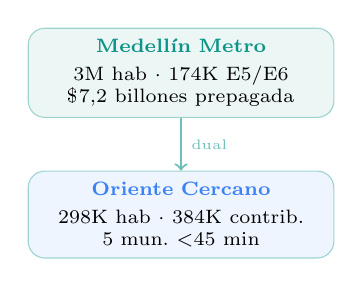
\begin{tikzpicture}[
  mkt/.style={draw=mercado!40, fill=white, rounded corners=6pt,
              text width=3.6cm, minimum height=1.1cm, align=center,
              font=\scriptsize, inner sep=4pt},
]
\node[mkt, fill=mercado!8] (m1) at (0,0) {
  \textcolor{mercado}{\textbf{Medellín Metro}}\\[2pt]
  {\scriptsize 3M hab $\cdot$ 174K E5/E6\\
  \$7,2 billones prepagada}
};
\node[mkt, fill=velocidad!8] (m2) at (0,-1.8) {
  \textcolor{velocidad}{\textbf{Oriente Cercano}}\\[2pt]
  {\scriptsize 298K hab $\cdot$ 384K contrib.\\
  5 mun.\ $<$45 min}
};
\draw[->, thick, mercado!60] (m1) -- node[right, font=\tiny\color{mercado}] {dual} (m2);
\end{tikzpicture}
\end{columns}

\vspace{4pt}
{\tiny\textcolor{riesgo}{Fuentes: Catastro Municipal (bp59-rj8r), DANE CNPV 2018, RUAF Aseguramiento, Supersalud}}
\end{frame}

% ============================================================
% SLIDE 3: BRECHA
% ============================================================
{
\setbeamercolor{background canvas}{bg=brecha!3}
\begin{frame}{\eqvar{brecha}{Brecha}: 0,54 camas por cada 1.000 habitantes}

\begin{columns}[T]
\column{0.50\textwidth}
\vspace{-2pt}

{\footnotesize\textbf{Dato 1: Déficit crítico en todo el Valle de Aburrá}}

\vspace{4pt}
{\scriptsize
Medellín tiene \textcolor{brecha}{\textbf{0,54 camas/1.000 hab}}. La OMS recomienda 3 a 5. El corredor Las Palmas tiene \textcolor{brecha}{\textbf{cero}} servicios ambulatorios especializados y \textcolor{brecha}{\textbf{cero}} camas de alta complejidad.
}

\vspace{8pt}
{\footnotesize\textbf{Dato 2: 103.913 habitantes sin cobertura al 2037}}

\vspace{4pt}
{\scriptsize
DENSURBAM (URBAM-EAFIT) proyecta \textbf{103.913 hab} en el corredor al 2037 sin cobertura de salud. Se requieren \textbf{363.696 m²} de equipamiento. Hoy hay \textcolor{brecha}{\textbf{0,0 m²/hab}}. IRS Salud El Poblado: \textcolor{brecha}{\textbf{0,27}} vs umbral 2,5.
}

\column{0.46\textwidth}
\vspace{4pt}
{\scriptsize
\begin{tabular}{@{}lcc@{}}
\toprule
\textbf{Zona} & \textbf{Camas/1000} & \textbf{Déficit} \\
\midrule
\rowcolor{brecha!10}
Medellín & \textcolor{brecha}{\textbf{1.0}} & --67\% \\
\rowcolor{brecha!10}
Envigado & \textcolor{brecha}{\textbf{0.6}} & --80\% \\
\rowcolor{brecha!10}
Sabaneta & \textcolor{brecha}{\textbf{0.5}} & --83\% \\
\rowcolor{brecha!15}
\textbf{Corredor L.P.} & \textcolor{brecha}{\textbf{0.0}} & \textcolor{brecha}{\textbf{--100\%}} \\
\midrule
OMS mínimo & 3.0 & --- \\
\bottomrule
\end{tabular}
}

\vspace{6pt}

\begin{tikzpicture}
  \fill[brecha!20] (0,0) rectangle (0.27/2.5*4.5, 0.4);
  \node[right, font=\scriptsize\bfseries\color{brecha}] at (0.27/2.5*4.5+0.1, 0.2) {El Poblado: 0.27};
  \draw[brecha, thick, dashed] (2.5/2.5*4.5, -0.1) -- (2.5/2.5*4.5, 0.6);
  \node[font=\tiny\color{brecha}, anchor=south] at (2.5/2.5*4.5, 0.6) {Umbral: 2.5};
\end{tikzpicture}
\end{columns}

\vspace{2pt}
{\tiny\textcolor{riesgo}{Fuentes: REPS (s2ru-bqt6), DENSURBAM (URBAM-EAFIT/AMVA), DANE}}
\end{frame}
}

% ============================================================
% SLIDE 4: VELOCIDAD
% ============================================================
\begin{frame}{\eqvar{velocidad}{Velocidad}: edificio existente, 18--24 meses para abrir}

\begin{columns}[T]
\column{0.50\textwidth}
\vspace{-2pt}

{\footnotesize\textbf{Dato 1: Access Point ya está construido}}

\vspace{4pt}
{\scriptsize
Proyecto de Acierto Inmobiliario en Km 7 Vía Las Palmas: \textbf{4 torres, 10 pisos, 1.085 parqueaderos}. No hay que construir --- solo adecuar. Fit-out médico: \textcolor{velocidad}{\textbf{18--24 meses}} vs 54+ meses de construcción greenfield.
}

\vspace{8pt}
{\footnotesize\textbf{Dato 2: CAPEX \$67.000 millones, apertura H1 2028}}

\vspace{4pt}
{\scriptsize
Inversión Fase 1: \textbf{\$67.000M COP} (adecuación + RMN 3T + TAC + 4 quirófanos + IT). Sin terreno, sin construcción. PET-CT en Fase 2 (\$14.000M) cuando el volumen lo justifique.
}

\column{0.46\textwidth}
\vspace{4pt}
{\scriptsize
\begin{tabular}{@{}lcc@{}}
\toprule
& \textbf{Access Point} & \textbf{Greenfield} \\
\midrule
\rowcolor{velocidad!8}
CAPEX & \textcolor{velocidad}{\textbf{\$67.000M}} & \$250.000M+ \\
\rowcolor{velocidad!8}
Timeline & \textcolor{velocidad}{\textbf{18--24 meses}} & 54+ meses \\
Construcción & No & Sí \\
\rowcolor{velocidad!8}
Terreno & Arriendo & Compra \\
\rowcolor{velocidad!8}
Apertura & \textcolor{velocidad}{\textbf{H1 2028}} & 2031+ \\
\bottomrule
\end{tabular}
}

\vspace{6pt}
{\scriptsize
\textcolor{velocidad}{\textbf{¿Por qué \#2 y no \#1?}}\\[2pt]
Las Palmas Bajo lidera el MCDA (88 vs 78). Pero requiere lote + diseño + obra = 54+ meses. \textbf{Access Point es la decisión de velocidad.}
}
\end{columns}

\vspace{2pt}
{\tiny\textcolor{riesgo}{Nota: 18--24 meses incluye diseño interior, refuerzo estructural (RMN 15 ton), blindaje RF, habilitación REPS, permisos INVIMA.}}
\end{frame}

% ============================================================
% SLIDE 5: MARCA
% ============================================================
\begin{frame}{\eqvar{marca}{Marca}: el único JCI de Antioquia, 55 años de reputación}

\begin{columns}[T]
\column{0.50\textwidth}
\vspace{-2pt}

{\footnotesize\textbf{Dato 1: Único JCI en Antioquia}}

\vspace{4pt}
{\scriptsize
HPTU es una de \textbf{solo 6 instituciones} con acreditación JCI en toda Colombia. Es la \textcolor{marca}{\textbf{única en Antioquia}}. Cero instituciones JCI están a menos de 30 minutos del Aeropuerto SKRG. Con la sede ambulatoria: \textbf{$\sim$25 min post-Túnel}.
}

\vspace{8pt}
{\footnotesize\textbf{Dato 2: Modelo Cleveland Clinic}}

\vspace{4pt}
{\scriptsize
Cleveland Clinic opera \textbf{270 centros ambulatorios} fuera del campus principal. Revenue ambulatorio: \textbf{USD \$6.800M} (43\% del total). Cada satélite hereda marca, protocolos y especialistas. \textcolor{marca}{\textbf{Heritage de marca}} = tarifas premium.
}

\column{0.46\textwidth}
\vspace{4pt}
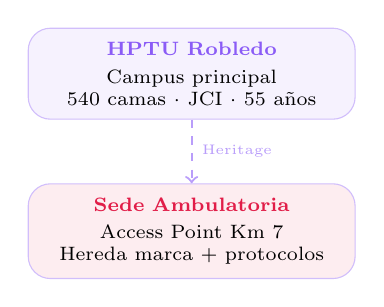
\begin{tikzpicture}[
  box/.style={draw=marca!40, fill=white, rounded corners=8pt,
              text width=3.8cm, minimum height=1cm, align=center,
              font=\scriptsize, inner sep=5pt},
]
\node[box, fill=marca!8] (campus) at (0,0) {
  \textcolor{marca}{\textbf{HPTU Robledo}}\\[2pt]
  Campus principal\\540 camas $\cdot$ JCI $\cdot$ 55 años
};
\node[box, fill=rose!8] (satelite) at (0,-2) {
  \textcolor{rose}{\textbf{Sede Ambulatoria}}\\[2pt]
  Access Point Km 7\\Hereda marca + protocolos
};
\draw[->, thick, marca!60, dashed] (campus) -- node[right, font=\tiny\color{marca}] {Heritage} (satelite);
\end{tikzpicture}

\vspace{6pt}
{\scriptsize\textcolor{marca}{\textbf{Diferenciación vs competencia:}}\\
Ningún competidor tiene JCI + portafolio de 7 categorías + captación del Oriente.}
\end{columns}
\end{frame}

% ============================================================
% SLIDE 6: EL RESULTADO
% ============================================================
{
\setbeamercolor{background canvas}{bg=resultado!3}
\begin{frame}{\eqvar{resultado}{Resultado}: \$51.000M/año, EBITDA 18\%, payback 6--8 años}

\vspace{4pt}
\begin{center}
{\small
\begin{tabular}{@{}lcccl@{}}
\toprule
\textbf{Escenario} & \textbf{Revenue/año} & \textbf{EBITDA} & \textbf{Payback} & \textbf{Nota} \\
\midrule
\rowcolor{brecha!6}
Pesimista (70\%) & \$35.700M & 15\% & $\sim$12 años & Ramp-up lento, baja captación \\
\rowcolor{resultado!12}
\textbf{Base (100\%)} & \textcolor{resultado}{\textbf{\$51.000M}} & \textcolor{resultado}{\textbf{18\%}} & \textcolor{resultado}{\textbf{$\sim$7 años}} & \textbf{6 líneas de servicio a madurez} \\
\rowcolor{velocidad!6}
Optimista (+Fase 2) & \$58.650M & 22\% & $\sim$5 años & Incluye PET-CT \\
\bottomrule
\end{tabular}
}
\end{center}

\vspace{8pt}
\begin{columns}[T]
\column{0.48\textwidth}
{\scriptsize\textbf{Revenue por línea (año maduro):}}

\vspace{2pt}
{\scriptsize
\begin{tabular}{@{}lr@{}}
Imágenes (TAC, RMN) & \$15.000M \\
Cirugía ambulatoria (4 ORs) & \$14.000M \\
Consulta especializada & \$8.000M \\
Chequeo ejecutivo / wellness & \$6.000M \\
Rehabilitación + oncología & \$5.000M \\
Estética / dermatología & \$3.000M \\
\end{tabular}
}

\column{0.48\textwidth}
{\scriptsize\textbf{Ventaja ambulatoria:}}

\vspace{2pt}
{\scriptsize
\begin{tabular}{@{}lcc@{}}
& \textbf{Ambulat.} & \textbf{Hospital} \\
\midrule
Margen EBITDA & \textcolor{resultado}{\textbf{18--22\%}} & 5--8\% \\
Payback & 6--8 años & 10--12 años \\
Competencia & Complem. & Directa \\
\end{tabular}

\vspace{4pt}
Arriendo: \$3.240M/año (35\% del EBITDA).\\
Ramp-up: Y1=40\%, Y2=65\%, Y3=85\%, Y4=100\%.
}
\end{columns}
\end{frame}
}

% ============================================================
% SLIDE 7: EL PORTAFOLIO
% ============================================================
\begin{frame}{7 categorías ambulatorias. Cero camas.}

\begin{columns}[T]
\column{0.48\textwidth}
\vspace{-2pt}

{\footnotesize\textcolor{mercado}{\textbf{Lo que SÍ incluye:}}}

\vspace{4pt}
{\scriptsize
\begin{enumerate}\setlength{\itemsep}{3pt}
  \item \textbf{Imágenes diagnósticas} — TAC, RMN 3T, ecografía, mamografía
  \item \textbf{Consulta especializada} — 10+ especialidades rotando desde Robledo
  \item \textbf{Cirugía ambulatoria} — 4 quirófanos: ortopedia, urología, ORL, ginecología
  \item \textbf{Chequeo ejecutivo / wellness} — Target: Zona Franca (12K empleados)
  \item \textbf{Rehabilitación} — Neuro, cardíaca, deportiva (inexistente en Oriente)
  \item \textbf{Estética / dermatología} — Turismo médico (23.323 pac/año)
  \item \textbf{Oncología ambulatoria} — QT, inmunoterapia, segunda opinión
\end{enumerate}
}

\column{0.48\textwidth}
\vspace{-2pt}

{\footnotesize\textcolor{brecha}{\textbf{Lo que NO incluye:}}}

\vspace{6pt}
{\scriptsize
\begin{itemize}\setlength{\itemsep}{4pt}
  \item[\textcolor{brecha}{$\times$}] Urgencias 24/7
  \item[\textcolor{brecha}{$\times$}] Hospitalización (camas)
  \item[\textcolor{brecha}{$\times$}] Unidad de Cuidados Intensivos
  \item[\textcolor{brecha}{$\times$}] Trasplantes
  \item[\textcolor{brecha}{$\times$}] Alta complejidad
\end{itemize}
}

\vspace{8pt}
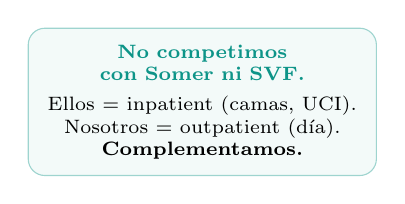
\begin{tikzpicture}
\node[draw=mercado!40, fill=mercado!5, rounded corners=6pt,
      text width=4cm, align=center, font=\scriptsize, inner sep=6pt] {
  \textcolor{mercado}{\textbf{No competimos con Somer ni SVF.}}\\[3pt]
  Ellos = inpatient (camas, UCI).\\
  Nosotros = outpatient (día).\\
  \textbf{Complementamos.}
};
\end{tikzpicture}
\end{columns}
\end{frame}

% ============================================================
% SLIDE 8: LA COMPETENCIA
% ============================================================
{
\setbeamercolor{background canvas}{bg=rose!3}
\begin{frame}{Ventana 2026--2028: la competencia ya se está moviendo}

\begin{columns}[T]
\column{0.50\textwidth}
\vspace{-2pt}

{\footnotesize\textbf{Dato 1: Competencia local a menos de 3 km}}

\vspace{3pt}
{\scriptsize
\begin{tabular}{@{}lrl@{}}
\toprule
\textbf{Centro} & \textbf{Dist.} & \textbf{Amenaza} \\
\midrule
\rowcolor{brecha!8}
Torre Oviedo & 2.65 km & \textcolor{brecha}{\textbf{Directa}} \\
Cl.\ Rosario & 0.93 km & Alta \\
\rowcolor{brecha!6}
BlueCare & 1.46 km & Media \\
\bottomrule
\end{tabular}

\vspace{3pt}
Campestre abrió sede Rionegro (mar 2026, \$30.000M, 250 pac/día). SVF va a 500 camas + helipuerto.
}

\column{0.46\textwidth}
\vspace{-2pt}

{\footnotesize\textbf{Dato 2: Nuestra diferenciación}}

\vspace{4pt}
{\scriptsize
\begin{itemize}\setlength{\itemsep}{2pt}
  \item \textcolor{marca}{\textbf{JCI}} — único en Antioquia
  \item \textcolor{marca}{\textbf{Heritage}} — 55+ años HPTU
  \item \textcolor{mercado}{\textbf{Portafolio}} — 7 categorías (vs 1--2 competidores)
  \item \textcolor{velocidad}{\textbf{Oriente}} — captación de 298K que nadie más alcanza
\end{itemize}

\vspace{4pt}
\textcolor{rose}{\textbf{Si HPTU no actúa en 2026--2028,}} el nicho ambulatorio premium será ocupado por Campestre, Quironsalud o un jugador internacional.
}
\end{columns}
\end{frame}
}

% ============================================================
% SLIDE 9: LO QUE FALTA
% ============================================================
\begin{frame}{Seis preguntas que debemos responder antes de decidir}

\vspace{-2pt}
{\scriptsize
\begin{tabular}{@{}cp{7cm}p{4cm}@{}}
\toprule
\textbf{\#} & \textbf{Pregunta} & \textbf{Próximo paso} \\
\midrule
\rowcolor{resultado!6}
1 & ¿Acierto Inmobiliario quiere un inquilino médico? & Reunión exploratoria --- abril \\
2 & ¿El edificio soporta una RMN de 15 toneladas? & Inspección estructural \\
\rowcolor{resultado!6}
3 & ¿SURA contrataría la sede ambulatoria? & Sondeo con dirección de red \\
4 & ¿Los pacientes elegirían Km 7 sobre opciones locales? & Encuestas de intención \\
\rowcolor{resultado!6}
5 & ¿El Túnel 2da etapa llega en H2 2027? & Monitoreo trimestral ANI \\
6 & ¿Los estratos del Oriente son dato real o proxy? & Solicitar datos a alcaldías \\
\bottomrule
\end{tabular}
}

\vspace{4pt}
\begin{center}

\begin{tikzpicture}
\node[draw=mercado!50, fill=mercado!5, rounded corners=6pt,
      text width=12cm, align=center, font=\scriptsize, inner sep=5pt] {
  \textcolor{mercado}{\textbf{Condiciones:}} (1) Factibilidad estructural \quad (2) Acuerdo Acierto Inmobiliario \quad (3) Pre-acuerdo aseguradora
};
\end{tikzpicture}
\end{center}
\end{frame}

% ============================================================
% SLIDE 10: LA DECISIÓN
% ============================================================
{
\setbeamercolor{background canvas}{bg=hptu}
\setbeamercolor{normal text}{fg=white}
\usebeamercolor[fg]{normal text}
\begin{frame}[plain]
\vfill
\begin{center}
{\Large\bfseries\textcolor{white}{Sede Ambulatoria HPTU en Access Point}}

\vspace{10pt}
\begin{tikzpicture}
  \draw[white, line width=0.5pt] (0,0) -- (8,0);
\end{tikzpicture}

\vspace{10pt}
\begin{tikzpicture}[
  box/.style={draw=white!30, fill=white!10, rounded corners=6pt,
              text width=3.2cm, minimum height=1.3cm, align=center,
              font=\scriptsize\color{white}, inner sep=5pt},
]
\node[box] at (0,0) {
  \textbf{¿Por qué Access Point?}\\[2pt]
  {\tiny Nodo puente 3M + 298K\\42K veh/día · $\sim$25 min aero.}
};
\node[box] at (4,0) {
  \textbf{¿Por qué ambulatorio?}\\[2pt]
  {\tiny Complementa Somer+SVF\\Margen $>$2$\times$ inpatient}
};
\node[box] at (8,0) {
  \textbf{¿Por qué ahora?}\\[2pt]
  {\tiny Campestre ya en Oriente\\Túnel H2 2027 · H1 2028}
};
\end{tikzpicture}

\vspace{8pt}
{\footnotesize\textcolor{white!85}{\textbf{Próximos pasos:}}\quad
\textcolor{white!70}{\scriptsize\textbf{1.} Visita Access Point \quad
\textbf{2.} POT + estructura \quad
\textbf{3.} Sondeo SURA}}

\vspace{8pt}
{\scriptsize\textcolor{white!50}{CAPEX \$67.000M $\cdot$ Revenue \$51.000M $\cdot$ EBITDA 18\% $\cdot$ Payback 6--8 años $\cdot$ H1 2028}}

\vspace{4pt}
{\tiny\textcolor{white!30}{hptu-localizacion.vercel.app}}
\end{center}
\begin{tikzpicture}[remember picture, overlay]
  \node[anchor=south] at ([yshift=10pt]current page.south) {
    
\includegraphics[height=0.9cm]{basica-white.png}
  };
\end{tikzpicture}
\vfill
\end{frame}
}

\end{document}
